\section{Simple bias configuration}
The circuit given in Figure \ref{lab3_ex5_de} is known as a simple kind of NPN bias configuration. First, students simulate the circuit with two values of RC, respectively 10 Ohms and 1k Ohms. Then, give your statement on the change of the current $I_E$ and explain the phenomena.
\begin{figure}[h]
    \centering
    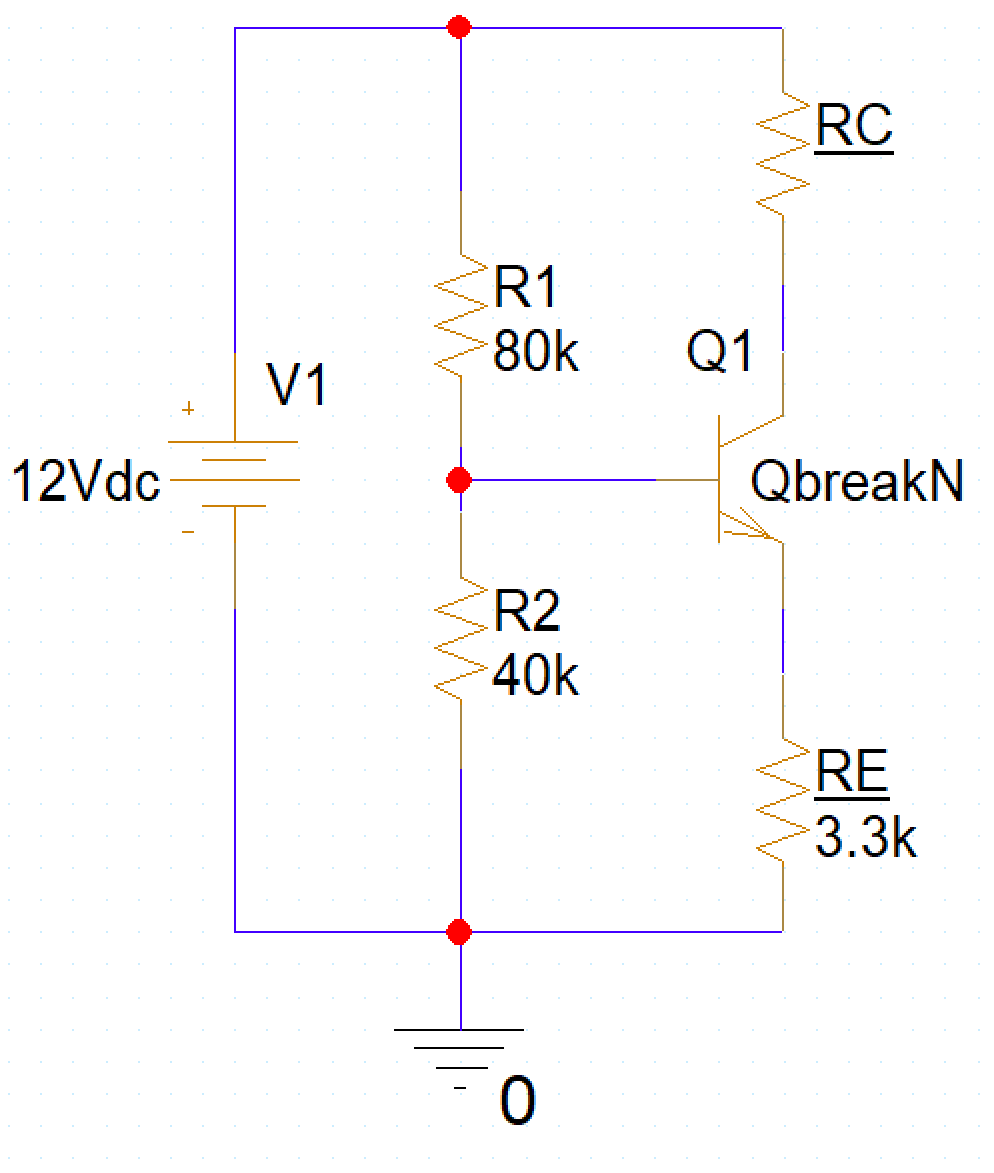
\includegraphics[width=8cm]{graphics/ex5/f1.png}
    \caption{Simple bias configuration}
    \label{lab3_ex5_de}
\end{figure}
\pagebreak
\subsection{Simulation}
\textbf{\textit{Your images go here (2 images)}}\\
\textbf{\textit{Step 1}}: Simulate the circuit with $R_C$ = 10 Ohms.\\
\textbf{\textit{Step 2}}: Simulate the circuit with $R_C$ = 1k Ohms.

\begin{figure}[ht]
    \centering
    \begin{subfigure}[b]{0.45\textwidth}
        \centering
        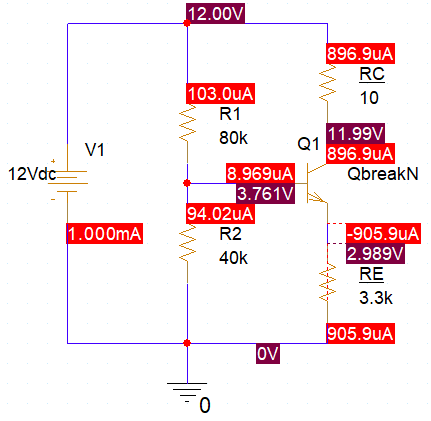
\includegraphics[width=\textwidth]{graphics/ex5/f2.PNG}
        \caption*{\(R_C=10\,\Omega\)}
    \end{subfigure}
    \hfill
    \begin{subfigure}[b]{0.45\textwidth}
        \centering
        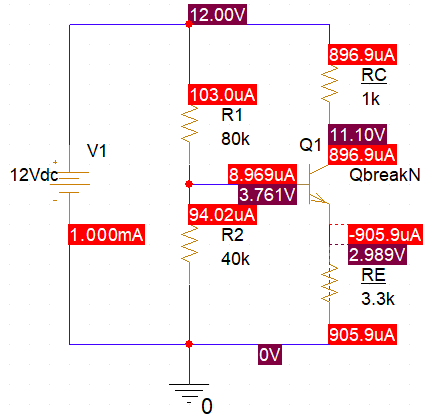
\includegraphics[width=\textwidth]{graphics/ex5/f3.PNG}
        \caption*{\(R_C=1\,\text{k}\Omega\)}
    \end{subfigure}
    \caption{Result from simulation}
\end{figure}

Nhận xét: Giá trị $I_E$ không thay đổi
\subsection{Circuit analysis}
Conduct some theoretical calculation to explain for the phenomena you have observed
from the simulation.

Theo định lý Thevenin, ta có mạch tương đương:
\begin{figure}[h]
    \centering
    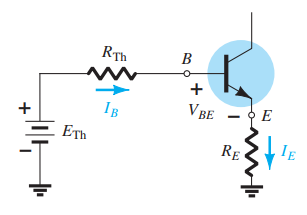
\includegraphics[width=0.3\textwidth]{graphics/ex5/f4.PNG}
\end{figure}

\pagebreak
\[
R_{TH} = \frac{R_1 \cdot R_2}{R_1 + R_2} = \frac{80\,k \cdot 40\,k}{80\,k + 40\,k} = 26.66 \, k\Omega
\]
\[
E_{TH} = \frac{V_{CC}}{R_1 + R_2} \cdot R_2 = \frac{12}{80\,k + 40\,k} \cdot 40\,k = 4 \, (\text{V})
\]
Theo Ohm's Law, KCL, KVL:
\[
E_{TH} = R_{TH} \cdot I_B + V_{BE} + R_E \cdot I_E \quad (1)
\]
\[
I_E = (\beta + 1) I_B \quad (2)
\]
Từ (1) và (2) ta có:
\[
I_E = \frac{(E_{TH} - V_{BE}) \cdot (\beta + 1)}{R_{TH} + (\beta + 1) R_E}
\]

Vậy, $I_E$ không phụ thuộc vào $R_C$ 